% ---
% Capitulo de revisão de literatura
% ---


\chapter{Referencial Teórico}\label{ch:referencial_teorico}


\section{Autenticação}\label{sec:autenticacao}
Autenticação é o processo que verifica a autenticidade de um usuário, processo ou dispositivo.
Essa verificação confirma a legitimidade da entidade em questão.
Durante a autenticação, a parte que examina assegura que a entidade sendo verificada é genuína, e esta última participa ativamente na troca de informações~\cite{usmonov2021identification}.

Para~\cite{dos2019tecnologias} existem três tipos de autenticação:

\begin{itemize}
    \item \textbf{Baseada em conhecimento:} utiliza informações que a pessoa sabe, como uma senha.
    \item \textbf{Com base em algo que a pessoa possua}, como um token ou cartão inteligente.
    \item \textbf{Com base em características físicas da pessoa}, também conhecidas como biometria.
\end{itemize}

Dos tipos citados, a biometria é considerada o método mais seguro, pois suas características físicas não podem ser roubadas, emprestadas ou esquecidas.
Forjar a autenticação biométrica é complexo e impraticável, já que mede aspectos únicos do indivíduo, como íris, retina, mão, características faciais e impressões digitais~\cite{dos2019tecnologias}.


\section{Biometria}\label{sec:biometria}
O termo \("\)biometria\("\) vem das palavras gregas \("\)bios\("\) (vida) e \("\)metrikos\("\) (medida)~\cite{magalhaes2003biometria}.
É o estudo que visa identificar um indivíduo com base em suas características fisiológicas e comportamentais~\cite{handa2019comparative}, ou seja, biometria é uma forma de identificar pessoas usando características físicas ou comportamentais únicas.

\subsection{Tecnologias Biométricas}\label{subsec:biometria-tecnologias}

\subsubsection{Reconhecimento facial}\label{subsec:reconhecimento-facial}
É uma tecnologia capaz de identificar uma pessoa a partir de uma imagem digital ou de um vídeo, de modo que é comparado as características faciais selecionadas de uma determinada imagem com os rostos existentes num banco de dados~\cite{orvalho2019reconhecimento}.

%\section{Aplicações Nativas vs. Híbridas}\label{sec:aplicacoes-nativas-vs.-hibridas}
%Aplicações nativas são aplicações escritas tendo em vista a execução em apenas um sistema operacional\cite{clow2019flutter}.
%Sendo assim, caso seja necessário desenvolver a mesma aplicação para Android e iOS, será preciso alocar duas equipes diferentes, com requisitos computacionais diferentes e habilidades distintas, para escrever e manter a aplicação em ambos SOs.
%
%Para os dois sistemas operacionais mais utilizados, aqui abordados, as linguagens de programação para desenvolvimento nativo de aplicações são Java \footnote{https://developer.android.com/docs} e Kotlin \footnote{https://developer.android.com/kotlin} para Android, e Objective-C \footnote{https://developer.apple.com/library/archive/documentation/Cocoa/Conceptual/ \newline ProgrammingWithObjectiveC/Introduction/Introduction.html} e Swift \footnote{https://developer.apple.com/swift/} para iOS\@.
%
%
%Para se desenvolver aplicações nativas para iOS é preciso utilizar o programa XCode \footnote{https://developer.apple.com/xcode/} que apenas está disponível em computadores com sistema operacional Mac OS instalado\cite{goadrich2011smart}.
%Este é um dos maiores motivos que impedem o desenvolvimento para iOS, a falta da diversidade de \textit{hardware} e \textit{software}, os quais possibilitam a programação e execução de testes, implicando em um gasto acima da média do que as empresas ou as pessoas físicas têm capacidade de investir.
%
%Diferentemente do desenvolvimento para iOS, é possível programar para Android na maioria dos sistemas operacionais utilizados atualmente, são eles: Windows, Sistemas Linux e Mac OS X~\cite{goadrich2011smart}.
%
%
%Com o passar dos anos, diversos tipos de tecnologias de desenvolvimento híbrido surgiram e cada vez mais foram aperfeiçoadas, tendo em vista que nem sempre há a possibilidade ou a viabilidade de escrever programas móveis de forma nativa.
%As tecnologias híbridas foram divididas em duas classificações: ferramentas que utilizam bibliotecas nativas e as que não as utilizam~\cite{clow2019flutter}.
%
%As ferramentas que usam bibliotecas nativas, começaram a aplicar uma API (\textit{Application Programming Interface}) unificada executada por cima do SDK (\textit{Software Development Kit}) nativo fornecido pela Google e Apple.
%A exemplo destas ferramentas, pode-se citar Xamarin, bastante conhecida e eventualmente ainda encontrada em utilização.
%Com Xamarin, é possível escrever códigos que podem ser executados em três tipos diferentes de SOs: Android, iOS e Windows Phone.
%Esta ferramenta possibilita escrever apenas um código utilizando a linguagem C\# \cite{petzold2015xamarin}.
%
%Porém, ao fazer uso de uma API unificada, o programador ainda precisa fazer escrita de código nativo de cada sistema operacional, pois a unificação não cobre todas as necessidades de programação das plataformas, muitas vezes tendo que possuir conhecimento de programação específica de cada sistema operacional para o qual se está desenvolvendo, e também, as aplicações finais pussuem uma aparência diferente umas das outras pelo fato de que é utilizada a interface gráfica (ou \textit{Widgets}) de cada SO~\cite{clow2019flutter}.
%
%As ferramentas que não fazem uso de bibliotecas nativas é o que hoje é conhecido como Web Apps.
%São aplicativos que são executados num browser dentro da aplicação numa tentativa de imitar a abordagem do SDK. Aplicações deste tipo são construídas com tecnologias web, possuindo implementações de HTML5 e Javascript.
%Contudo, o problema de se construir aplicações com esta tecnologia é a limitação da velocidade de internet, já que nem sempre um usuário possui a chance de estar conectado a uma rede com velocidade suficientemente rápida para que as aplicações sejam executadas de maneira aceitável, tornando-se muito lentas e caso não haja conexão de rede, a aplicação nem mesmo pode ser executada.
%A tecnologia de desenvolvimento chamada PhoneGap \footnote{https://phonegap.com/} é um exemplo bastante conhecido desta tecnologia~\cite{clow2019flutter}.
%
%Com o tempo, as tecnologias foram aperfeiçoadas tentando sempre cobrir os gargalos previamente apresentadas nas tecnologias existentes.
%As abordagens de desenvolvimento atualmente utilizadas e disputam entre si são React Native, da empresa de tecnologia Facebook e Flutter da Google.
%Estes dois frameworks trabalham com o suporte ao paradigma de programação reativa.
%Ou seja, são ferramentas que se propõe a lidar com a mudança de estados dos componentes gerada pela atualização de dados\cite{lima2019avaliacao}.
%
%
%\section{React Native}\label{sec:react-native}
%
%React Native é uma combinação de desenvolvimento nativo com React, uma biblioteca JavaScript para construção de interfaces de usuário.
%Este \textit{framework} para desenvolvimento de aplicações móveis híbdridas é baseado no \textit{framework} React, como já mencionado, e seu intuito é facilitar a construção das interfaces de usuário.
%
%Aplicações construídas com este framework utilizam JavaScript, abaixo da camada JavaScript, há uma ponte e mais abaixo, a parte nativa do framework.
%Esta camada nativa possui uma RootView (contendo os objetos de interface de usuário da aplicação) e uma ponte de interface construída em Objective C para iOS, e Java para Android.
%Esta ponte de interface é intermediadora da parte nativa do framework e a ponte do nível acima, construída em C e C++~\cite{yatsenko2019comparative};
%
%A compilação do código dinâmico JavaScript para código nativo representativo ocorre em tempo de execução, o código restante é executado em uma máquina virtual que é encontrada dentro da própria aplicação.
%Os componentes nativos iOS e Android são controlados pelos códigos em JavaScript através de uma ponte, o que faz com que as aplicações geradas não possuem a mesma identidade visual~\cite{yatsenko2019comparative}.
%
%\begin{figure}[H]
%    \centering
%    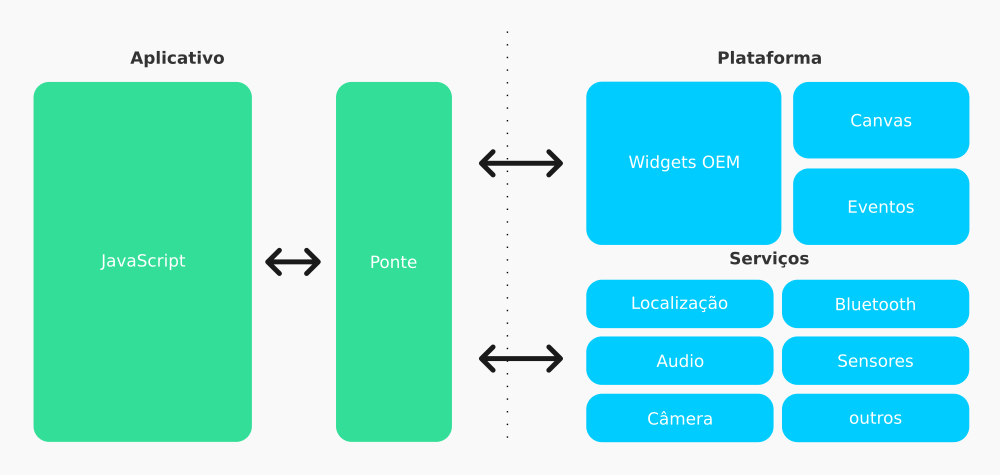
\includegraphics[width=15cm]{imagens/interacaoReactNative}
%    \caption{Interação do React Native com o Sistema Operacional}
%    Fonte: Adaptada de~\cite{yatsenko2019comparative}
%    \label{fig: Interação React Native SO}
%\end{figure}
%
%A Figura~\ref{fig: Interação React Native SO} apresenta a interação entre componentes nativos e o código em JavaScript.
%Há uma ponte entre o código e os componentes visuais nativos (Widgets OEM), resultando em uma interface de usuário construída com a aparência visual dos componentes nativos.
%
%
%\section{Flutter}\label{sec:flutter}
%
%Flutter é um \textit{framework} da Google para construção de aplicações nativas e reativas para dispositivos móveis que utilizam Android e iOS~\cite{zammetti2019practical}.
%Tem como objetivo oferecer um rápido desenvolvimento de aplicativos de alta performance e utilizando-se apenas uma base de código.
%Utiliza Dart, uma linguagem orientada a objetos também criada pela Google.
%Sua ferramenta de renderização é Skia 2D, que funciona em diversos tipos de \textit{hardware} e \textit{software} e também é uma ferramenta gerenciada pela mesma empresa de tecnologia, e está disponível para utilização pela licença BSD~\cite{napoli2019beginning}.
%
%
%A ferramenta de desenvolvimento Flutter foi apresentada recentemente, em 2017, e está se tornando uma opção atrativa no campo da programação para dispositivos móveis, já que possui uma abordagem de desenvolvimento híbrido diferente das opções anteriormente apresentadas no mercado.
%Uma dessas vantagens sobre outras soluções é que, com Flutter, só é necessária uma base de código para ambos os sistemas operacionais, e isto implica em aplicativos com a mesma aparência, tanto em dispositivos Android como iOS\@.
%
%
%
%\begin{figure}[H]
%    \centering
%    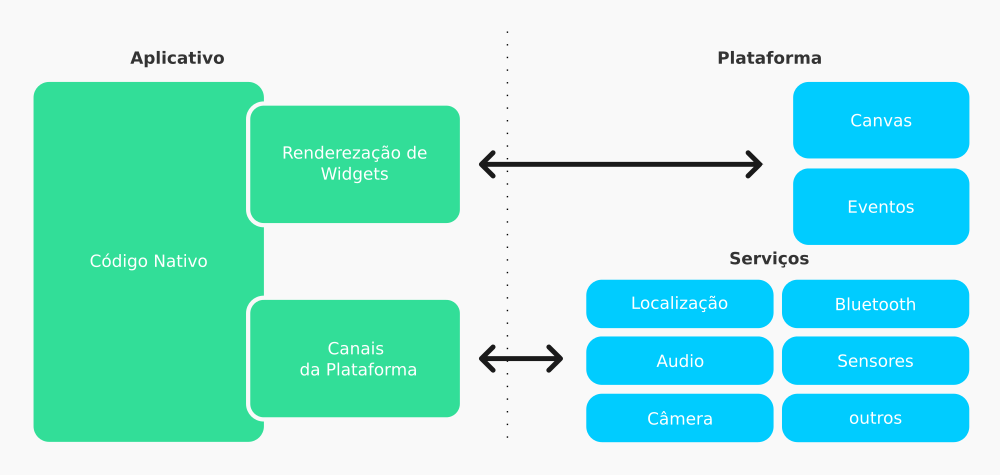
\includegraphics[width=15cm]{imagens/interacaoFlutter}
%    \caption{Interação do Flutter com o Sistema Operacional}
%    Fonte: Adaptada de~\cite{yatsenko2019comparative}
%    \label{fig: Interação Flutter SO}
%\end{figure}
%
%A interface de usuário é renderizada com os próprios componentes do \textit{framework}, como é ilustrado na Figura ~\ref{fig: Interação Flutter SO}, e é esse o motivo para a interface ser visualmente equivalente nos aplicativos de ambos sistemas operacionais, o que não ocorre na maioria das abordagens existentes, pois elas utilizam os componentes nativos.
%Isto afeta no momento da programação, pois um desenvolvedor Flutter não precisa se preocupar caso a interface de usuário, ou widgets, possuam suporte a estes componentes na camada nativa\cite{zammetti2019practical}.
%
%\subsection{Dart}\label{subsec:dart}
%
%A linguagem de programação Dart foi criada pela Google e foi otimizada para ser utilizada em diferentes plataformas~\cite{clow2019flutter}, como por exemplo no desenvolvimento para web, desktop, \textit{server-side} (aplicações para servidor) e para aplicações móveis~\cite{biessek2019dart}.
%Sua primeira versão estável foi apresentada em 2013, portanto, é uma abordagem que surgiu recentemente.
%
%É com a linguagem Dart que se desenvolvem aplicativos com o \textit{framework} Flutter, e foi escolhida pela Google para este fim por ser uma linguagem de alto-nível que combina os benefícios das linguagens mais maduras e foi concebida para substuir JavaScript, já que era focada no desenvolvimento para Web.
%Dart é uma linguagem robusta e flexível que possui funcionalidades de uma linguagem orientada a objetos.
%É estaticamente tipada, ou seja, os tipos são verificados em tempo de execução.
%Possui \textit{Garbage Collection}, que lida com alocação de memória, e realiza a limpeza, geralmente de objetos alocados que não estão mais em uso.
%Possui muitas outras funcionalidades que garantem uma melhor escrita de código~\cite{biessek2019dart}.
%
%Para muitos programadores, Dart pode parecer um desafio para o desenvolvimento por terem que aprender uma nova linguagem, porém, Dart não reinventa conceitos de programação, é baseado em conceitos já presentes em outras linguagens, porém de forma aprimorada para que haja a melhor efetividade da programação.
%Possui uma abordagem de simples entendimento pelo fato de que é inspirada nas liguagens mais conhecidas e utilizadas como Java, JavaScript e sua sintaxe é similar à linguagem C~\cite{clow2019flutter}.
%
%A execução de Dart acontece de duas maneiras, compilação \textit{Just-In-Time}, onde o código fonte é carregado e compilado em código de máquina nativo através da Máquina Virtual Dart em tempo de execução.
%É utilizada quando se está debugando o aplicativo peli emulador.
%E a segunda maneira é \textit{Ahead-Of-Time}, que ocorre quando a Máquina Virtual Dart e o código são pré-compilados, tendo-se a utilização do garbage collector e uma variedade métodos do SDK Dart na aplicação.
%Este tipo de execução ocorre quando a aplicação é lançada para utilização nas lojas de aplicativo, como Google Play e App Store~\cite{napoli2019beginning}.
%
%
%\section{Web Services}\label{sec:web-services}
%
%
%Hoje em dia, a maneira mais prática para realizar a troca de dados entre diferentes sistemas de informação é através dos chamados Web Services\cite{tihomirovs2016webservices}, que são tecnologias que permitem aplicações heterogêneas interajam entre si de forma que pareçam compatíveis\cite{eulalio2016webservices}.
%
%
%SOA (\textit{Service-Oriented Architecture}), que em português significa Arquitetura Orientada a Serviços, é a especificação que trata da integração de sistemas de informação, e relata a maneira como os dados devem estar estruturados para transitarem entre estes sistemas\cite{eulalio2016webservices}.
%No cenário atual de desenvolvimento, são duas as formas de web services mais utilizadas, sendo eles o padrão SOAP (\textit{Simple Object Access Protocol}) e REST (\textit{Representational State Transfer Protocol}).
%
%SOAP usa protocolos de comunicação como HTTP (\textit{Hypertext Transfer Protocol}) e SMTP (\textit{Simple Mail Transfer Protocol}) para transporte de dados, os quais são enviados no formato XML (\textit{Extensible Markup Language}). Sua utilização ocorre da seguinte forma: um provedor de serviço publica a descrição de determinado serviço o qual pode ser encontrado pelo requisitante na forma de uma instância deste serviço.
%Tal padrão possui alguns problemas de desempenho causadas durante a formação das mensagens, onde são acrescentados cabeçalho e corpo adicionais à mensagem~\cite{tihomirovs2016webservices}.
%
%\begin{figure}[H]
%    \centering
%    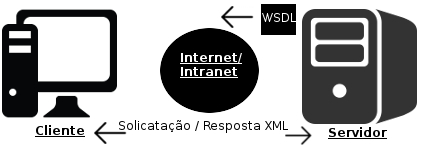
\includegraphics{imagens/soap}
%    \caption{Funcionamento Web Service SOAP}
%    Fonte~\cite{eulalio2016webservices}:
%    \label{fig: SOAP}
%\end{figure}
%
%A Figura~\ref{fig: SOAP}, apresenta a maneira como o padrão SOAP opera e é ilustrada da seguinte forma: as informações trocadas entre as partes transitam em XML, são descritas por meio de um arquivo WSDL (\textit{Web Services Description Language}), o qual relata onde determinado serviço pode ser encontrado, o tipo de dados, parâmentros e métodos que possui.
%
%
%Já o padrão REST é mais recente que a abordagem SOAP e usa o protocolo HTTP para a transmissão das informações, e seus dados podem transitar em diversos formatos, sendo o XML e JSON (\textit{JavaScript Object Notation}) os mais utilizados.
%Este padrão é relativamente mais leve que o anteriormente abordado\cite{tihomirovs2016webservices}, é bastante similar à abordagem SOAP no quesito objetivo, o diferencial do padrão REST está na redução da carga que SOAP possui devido ao WSDL\cite{eulalio2016webservices}.
%
%\begin{figure}[H]
%    \centering
%    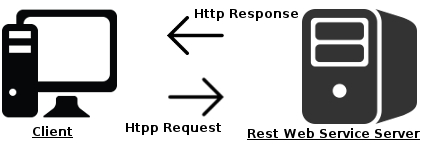
\includegraphics{imagens/rest}
%    \caption{Funcionamento Web Service REST}
%    Fonte~\cite{eulalio2016webservices}:
%    \label{fig: REST}
%\end{figure}
%
%Como anteriormente mencionado, e exemplificado na Figura~\ref{fig: REST}, a simplicidade do padrão REST está na ausência do arquivo WSDL, obrigatório no padrão SOAP. Com o REST, cada mensagem HTTP possui toda a informação necessária para que o cliente (responsável pela utilização do Web Service) realize a interpretação da requisição feita ao servidor, minimizando problemas na aplicação ao consumir tais informações\cite{eulalio2016webservices}.
%
%Portanto, ao se planejar o desenvolvimento de uma aplicação móvel que necessita consumir dados de integração de sistemas, é preciso definir um padrão de Web Service a ser utilizado.
%De acordo com~\cite{tihomirovs2016webservices}, aplicações que utilizam REST são as que demandam maior performance, escalabilidade e compatibilidade.
%Enquanto as que utilizam o padrão SOAP, são projetos que exigem maior nível de segurança e confiabilidade como aplicações bancárias e sistemas de pagamento.
%
%
%\section{Considerações Finais}\label{sec:consideracoes-finais}
%
%Neste capítulo foram abordados os principais conceitos envolvidos neste projeto, relacionados ao desenvolvimento de uma aplicação móvel, também são apresentadas as principais tecnologias para aplicações híbridas existentes e como se deu o processo de evolução dessas tecnologias, assim como as principais vantagens e desvantagens notadas ao se construir aplicativos utilizando-se tecnologias de desenvolvimento híbrido.
%Também foram apresentados conceitos do funcionamento da Arquitetura Orientada a Serviços e a maneira que ela proporciona uma melhor integração dos sistemas, possibilitando um fácil consumo de informações pelos aplicativos.
%
%No próximo capítulo será apresentado a metodologia de desenvolvimento deste trabalho e como se deu a formulação de estudo dos conteúdos necessários para a construção da aplicação proposta.